%%%%%%%%%%%%%%%%%%%%%%%%%%%%%%%%%%%%%%%%%
% CSAS 2026 Poster — EPAA: A Two-Stage Approach to
% Quantifying Scoring Talent in the NBA
%
% Based on the Jacobs Landscape Poster LaTeX Template
% Version 1.0 (29/03/13)
% License: CC BY-NC-SA 3.0
%%%%%%%%%%%%%%%%%%%%%%%%%%%%%%%%%%%%%%%%%

%----------------------------------------------------------------------------------------
% PACKAGES AND OTHER DOCUMENT CONFIGURATIONS
%----------------------------------------------------------------------------------------

\documentclass[final]{beamer}

\usepackage[size=custom,width=121.92,height=91.44,scale=1.24]{beamerposter} % 48x36

\usetheme{confposter}

\setbeamercolor{block title}{fg=dblue,bg=white}
\setbeamercolor{block body}{fg=black,bg=white}
\setbeamercolor{block alerted title}{fg=white,bg=dblue!70}
\setbeamercolor{block alerted body}{fg=black,bg=dblue!10}
\setbeamercolor{enumerate item}{fg=dblue}
\setbeamercolor{enumerate subitem}{fg=dblue}

\setbeamerfont{block title}{size=\Large,series=\bfseries}
\setbeamerfont{block body}{size=\normalsize}

\setbeamerfont{block alerted title}{size=\Large,series=\bfseries}
\setbeamerfont{block alerted body}{size=\normalsize}

\setbeamertemplate{caption}[numbered]

%-----------------------------------------------------------
% Define the column widths and overall poster size
% 3-column layout: sepwid = 0.024, onecolwid = 0.3, twocolwid = 0.624
%-----------------------------------------------------------

\newlength{\edgewid}
\newlength{\gutterwid}
\newlength{\onecolwid}

\setlength{\edgewid}{0.024\textwidth}    % left/right outer margins
\setlength{\gutterwid}{0.012\textwidth}  % gaps between columns
\setlength{\onecolwid}{0.309\textwidth}  % each content column
%\setlength{\bottommargin}{0.25in}

% \setlength{\topmargin}{-0.5in}

%-----------------------------------------------------------

\usepackage{graphicx}
\usepackage{booktabs}
\usepackage{amsmath}
\usepackage{amssymb}
\usepackage{hyperref}
\usepackage{qrcode}  % For QR code generation

%----------------------------------------------------------------------------------------
% TITLE SECTION
%----------------------------------------------------------------------------------------

% \title{A Two-Stage Approach to Quantifying NBA Scoring Talent}
%  
% \author{Alex Susi}
%  
% \institute{Georgia Institute of Technology}

%----------------------------------------------------------------------------------------
\setbeamertemplate{headline}{}
\newsavebox{\titlebox}
\begin{document}

\addtobeamertemplate{block end}{}{\vspace*{2ex}}
\addtobeamertemplate{block alerted end}{}{\vspace*{2ex}}

\setlength{\belowcaptionskip}{2ex}
\setlength\belowdisplayshortskip{2ex}



\begin{frame}[t]
\vspace*{1.27cm}

\savebox{\titlebox}{%
  \begin{minipage}{0.76\linewidth}
    \centering
    {\veryHuge\textbf{A Two-Stage Approach to Quantifying NBA Scoring Talent}}\\[1.2ex]
    {\huge Alex Susi}\\[0.4ex]
    {\Large Georgia Institute of Technology}
  \end{minipage}%
}

\begin{columns}[c,onlytextwidth]
  \begin{column}{0.12\linewidth}
    \centering
    
\includegraphics[height=1.5\ht\titlebox]{gaTech.png}
  \end{column}
  \begin{column}{0.76\linewidth}
    \centering
    \usebox{\titlebox}
  \end{column}
  \begin{column}{0.12\linewidth}
    \centering
    
\includegraphics[height=1.5\ht\titlebox]{nba.png}
  \end{column}
\end{columns}

\vspace{0.3cm}

\begin{center}
  \color{dblue}\rule{0.95\linewidth}{0.15cm}
\end{center}

\vspace{0.5cm}

\begin{columns}[t,totalwidth=\textwidth]

\begin{column}{\edgewid}\end{column}






%========================================================================================
% COLUMN 1
%========================================================================================

\begin{column}{\onecolwid}

%----------------------------------------------------------------------------------------
% INTRODUCTION
%----------------------------------------------------------------------------------------

\begin{alertblock}{Introduction}

The NBA is often referred to as a "make-or-miss" league. However, not all makes nor misses are created equal. A contested layup, an open midrange pull-up, and a wide open catch-and-shoot 3-pointer all have different expected conversion rates.

\vspace{2ex}

\begin{table}[ht]
\centering
%\begin{tabular}{lllrr}
\begin{tabular}{l@{\hspace{0.8em}}l@{\hspace{0.8em}}l@{\hspace{1em}}r@{\hspace{1em}}r}
\toprule
\textbf{Shot Type} & \textbf{Defense} & \textbf{Dribbles} & \textbf{N} & \textbf{FG\%} \\
\midrule
Rim & Tight   & 2 &   4,770 & 65.6 \\
Mid-range  & Open     & 1    &  2,407 & 45.7 \\
3-point  & Wide Open      & 0    & 35,293 & 38.3 \\
\bottomrule
\end{tabular}
\caption{Summary table by shot type, defender distance, and dribbles.}
\end{table}


\vspace{1ex}


Typical metrics such as FG\%, eFG\%, and TS\% conflate \textbf{shot quality} with \textbf{shooting skill}.

\vspace{2ex}

We introduce \textbf{Expected Points Above Average (EPAA)}, a framework that:

\begin{enumerate}
\item Estimates \textit{shot quality} using contextual features.
\item Estimates \textit{shooting talent} via Bayesian hierarchical modeling.
\end{enumerate}

\vspace{2ex}

By controlling for shot quality, closest defender, and team defense, \textbf{EPAA identifies the most proficient scorers with full posterior uncertainty}, allowing front offices and fans to more accurately assess scoring abilities. 

\vspace{2ex}

This work uses public NBA tracking data from over 200,000 field goal attempts during the 2024–25 regular season, accessed via the \texttt{hoopR} package.

\end{alertblock}





%----------------------------------------------------------------------------------------
% METHODOLOGY
%----------------------------------------------------------------------------------------

\begin{block}{Methodology}

\textbf{Stage 1: Shot Quality} \\[0.5ex]
\textit{"How hard was this shot for an average player guarded by an average defender?"}
\vspace{0.5ex}
\begin{itemize}
\item Expected Field Goal Percentage (xFG) is estimated using three XGBoost classifiers (one per shot type: rim, mid-range, 3-point), trained on play-by-play features.
\item Player and defender identities are intentionally excluded in this stage.
\end{itemize}

\vspace{2ex}

\textbf{Stage 2: Shooting Talent} \\[0.5ex]
\textit{"How good is each player at converting shots after controlling for shot quality?"}
\vspace{0.5ex}
\begin{itemize}
\item Modeled using a Bayesian hierarchical framework in Stan with random effects for shooters, individual defenders, and defensive teams.
\item Partial pooling shrinks lower-volume players toward the league mean while preserving separation for high-volume stars, producing skill parameters with uncertainty quantification rather than simple point estimates.
\end{itemize}




\end{block}



%----------------------------------------------------------------------------------------

\setbeamercolor{block alerted title}{fg=black,bg=norange}
\setbeamercolor{block alerted body}{fg=black,bg=white}
\begin{alertblock}{Code}
\begin{columns}[T]
  \begin{column}{0.6\linewidth}
  \vspace{2ex}
    \textbf{GitHub repo}: \texttt{github.com/alex-susi/exp-fg-pct} \\

    \vspace{2ex}

    \textbf{Pipeline:} R + Stan (\texttt{cmdstanr}) \\
    \vspace{2ex}
    
    \textbf{Artifacts}: Code, models, graphs, and output CSVs. \\
    \vspace{2ex}
%    \textbf{Scripts:} \texttt{01\_data\_pipeline.R} $\to$ \texttt{02\_xgb\_shot\_difficulty.R} $\to$ \texttt{03\_stan\_random\_effects.R} \\
    \textbf{Data:} NBA Stats API via \texttt{hoopR} \\
    \vspace{2ex}
    \textbf{Contact:} \texttt{alex.susi2298@gmail.com}


  \end{column}
  \begin{column}{0.35\linewidth}
    \centering
    \qrcode[height=5in]{https://github.com/alex-susi/exp-fg-pct}
  \end{column}
\end{columns}
\end{alertblock}



%----------------------------------------------------------------------------------------

\end{column}

%\begin{column}{\sepwid}\end{column}
\begin{column}{\gutterwid}\end{column}

%========================================================================================
% COLUMN 2
%========================================================================================

\begin{column}{\onecolwid}

%----------------------------------------------------------------------------------------
% SHOT QUALITY MODELS (STAGE 1)
%----------------------------------------------------------------------------------------

\begin{block}{Stage 1: Shot Quality}


Training the model across the 2024-25 season yields an xFG for every shot attempt. 

\vspace{2ex}

The SHAP plots highlight each feature's importance to xFG. A positive SHAP value corresponds to an increase in xFG. Feature importance varies across shot types.

\vspace{1ex}

\begin{figure}

\includegraphics[width=\linewidth]{shap_feature_importance.png}
\caption{\textbf{SHAP Feature Importance by Shot Type}. For rim attempts, defender distance and dunks explain most of the variability. Defender distance, shot clock, shot distance, and shot angle rank near the top for mid-range and 3-pointers.}
\end{figure}

\vspace{1ex}

Outputs from the Shot Quality model are transformed on the logit scale and used as a baseline in the Shooting Talent model.


\end{block}

%----------------------------------------------------------------------------------------

%----------------------------------------------------------------------------------------
% EPAA MODEL (STAGE 2)
%----------------------------------------------------------------------------------------

\begin{block}{Stage 2: Shooting Talent}

For each shot attempt $n = 1, \dots, N$, let:
\[
\begin{aligned}
  y_n &\in \{0,1\} & &\text{shot outcome (make/miss)} \\
  t_n &\in \{1,2,3\} & &\text{shot type (rim, mid-range, three-point)}
\end{aligned}
\]

\vspace{2ex}

\textbf{Likelihood and Linear Predictor}
\vspace{0.5ex}
\[
\begin{aligned}
  &y_n \sim \mathrm{Bernoulli}\!\bigl(\mathrm{logit}^{-1}(\eta_n)\bigr) \\
  &\eta_n = \underbrace{\alpha_{t_n}
    + \beta_{t_n} \cdot \mathrm{xfg\_logit}_n
    }_{\text{Shot Quality}}
    + \underbrace{a^{\mathrm{p}}_{j[n],\,t_n}
    }_{\text{shooter talent}}
    + \underbrace{a^{\mathrm{f}}_{d[n],\,t_n}
    }_{\substack{\text{individual} \\ \text{defender}}}
    + \underbrace{a^{\mathrm{m}}_{k[n],\,t_n}
    }_{\substack{\text{team} \\ \text{defense}}}
\end{aligned}
\]

\vspace{1.5ex}
\fcolorbox{dblue}{dblue!10}{%
  \parbox{0.95\linewidth}{%
    \textbf{Random effects} jointly model shooter skill, individual defender ability, and team defensive scheme --- three sources typically confounded in shooting metrics.
  }%
}
\vspace{1ex}

%The intercept $\alpha_t$ and slope $\beta_t$ recalibrate the Stage~1 output per shot type. Three sets of \textbf{random effects} decompose residual skill.

\vspace{3ex}

\textbf{Random Effects}
\vspace{0.5ex}
\[
\begin{aligned}
  a^{\mathrm{p}}_{j,t} &= \mu^{\mathrm{vol}}_t
    \cdot x^{\mathrm{vol}}_{j,t}
    + \sigma^{\mathrm{p}}_t \cdot z^{\mathrm{p}}_{j,t},
        &z^{\mathrm{p}}_{j,t}
    &\sim \mathcal{N}(0,\, 1) \text{ for all players } j = 1,\dots,J \\[4pt]
  a^{\mathrm{f}}_{d,t}
    &= \sigma^{\mathrm{f}}_t
    \cdot z^{\mathrm{f}}_{d,t},
        &z^{\mathrm{f}}_{d,t}
    &\sim \mathcal{N}(0,\, 1) \text{ for all defenders } d = 1,\dots,D  \\[4pt]
  a^{\mathrm{m}}_{k,t}
    &= \sigma^{\mathrm{m}}_t
    \cdot z^{\mathrm{m}}_{k,t},
        &z^{\mathrm{m}}_{k,t}
    &\sim \mathcal{N}(0,\, 1) \text{ for all teams } k = 1,\dots,K 
\end{aligned}
\]
\vspace{0.5ex}

where $x^{\mathrm{vol}}_{j,t}$ is standardized $\log(1 + \text{FGA per 36\,min})$ for player $j$ in shot type $t$.

\vspace{3ex}

\textbf{Priors}
\vspace{0.5ex}
\[
\begin{aligned}
  \alpha_t &\sim \mathcal{N}(0,\; 0.25^2)
    & \beta_t  &\sim \mathcal{N}^{+}(1,\; 0.25^2) \\[4pt]
  \mu^{\mathrm{vol}}_t &\sim \mathcal{N}(0,\; 0.3^2) \\[4pt]
  \sigma^{\mathrm{p}}_t
    &\sim \mathcal{N}^{+}\!\bigl(0,\; s^{\mathrm{p}}_t\bigr),
    &s^{\mathrm{p}}
    &= (0.30,\; 0.30,\; 0.25) \\
  \sigma^{\mathrm{f}}_t
    % &\sim \mathcal{N}^{+}(0,\; 0.20) \;\; \forall\, t \\
    &\sim \mathcal{N}^{+}\!\bigl(0,\; s^{\mathrm{f}}_t\bigr),
    &s^{\mathrm{f}}
    &= (0.20,\; 0.20,\; 0.20) \\
  \sigma^{\mathrm{m}}_t
    &\sim \mathcal{N}^{+}\!\bigl(0,\; s^{\mathrm{m}}_t\bigr),
    &s^{\mathrm{m}}
    &= (0.12,\; 0.10,\; 0.06)
\end{aligned}
\]

% {\small Family-specific prior scales encode basketball domain knowledge: $s^{\mathrm{player}}$ and $s^{\mathrm{team}}$ vary by shot family because defensive scheme effects are largest at the rim and smallest on threes, while individual defender impact ($\sigma^{\mathrm{def}}_t$) uses a common scale across all families. The half-normal $\mathcal{N}^{+}$ constrains variance parameters to be positive. The slope prior $\beta_t \sim \mathcal{N}^{+}(1, 0.25^2)$ is centered at the identity transform, encoding the belief that a better Stage~1 prediction should correspond to a higher make probability.}

\end{block}







\end{column}

%\begin{column}{\sepwid}\end{column}
\begin{column}{\gutterwid}\end{column}

%========================================================================================
% COLUMN 3
%========================================================================================

\begin{column}{\onecolwid}


%----------------------------------------------------------------------------------------
% RESULTS
%----------------------------------------------------------------------------------------

\begin{block}{Results}

\textbf{Player Leaderboards} 

\begin{figure}

\includegraphics[width=\linewidth]{player_caterpillar.png}
\caption{\textbf{Top 5 and Bottom 5 Players by EPAA per 100 shots}}
\end{figure}

\vspace{1.5ex}

\begin{figure}

\includegraphics[width=\linewidth]{defender_caterpillar.png}
\caption{\textbf{Top 5 and Bottom 5 Defenders by Defensive EPAA per 100 shots contested}}
\end{figure}

\vspace{1.5ex}

\begin{figure}
\begin{minipage}[t]{0.48\linewidth}
\centering

\includegraphics[width=\linewidth]{twostage_calibration.png}
\caption{\textbf{Model Calibration}. Tight adherence to the 45-degree line confirms model calibration.}
\end{minipage}
\hfill
\begin{minipage}[t]{0.48\linewidth}
\centering
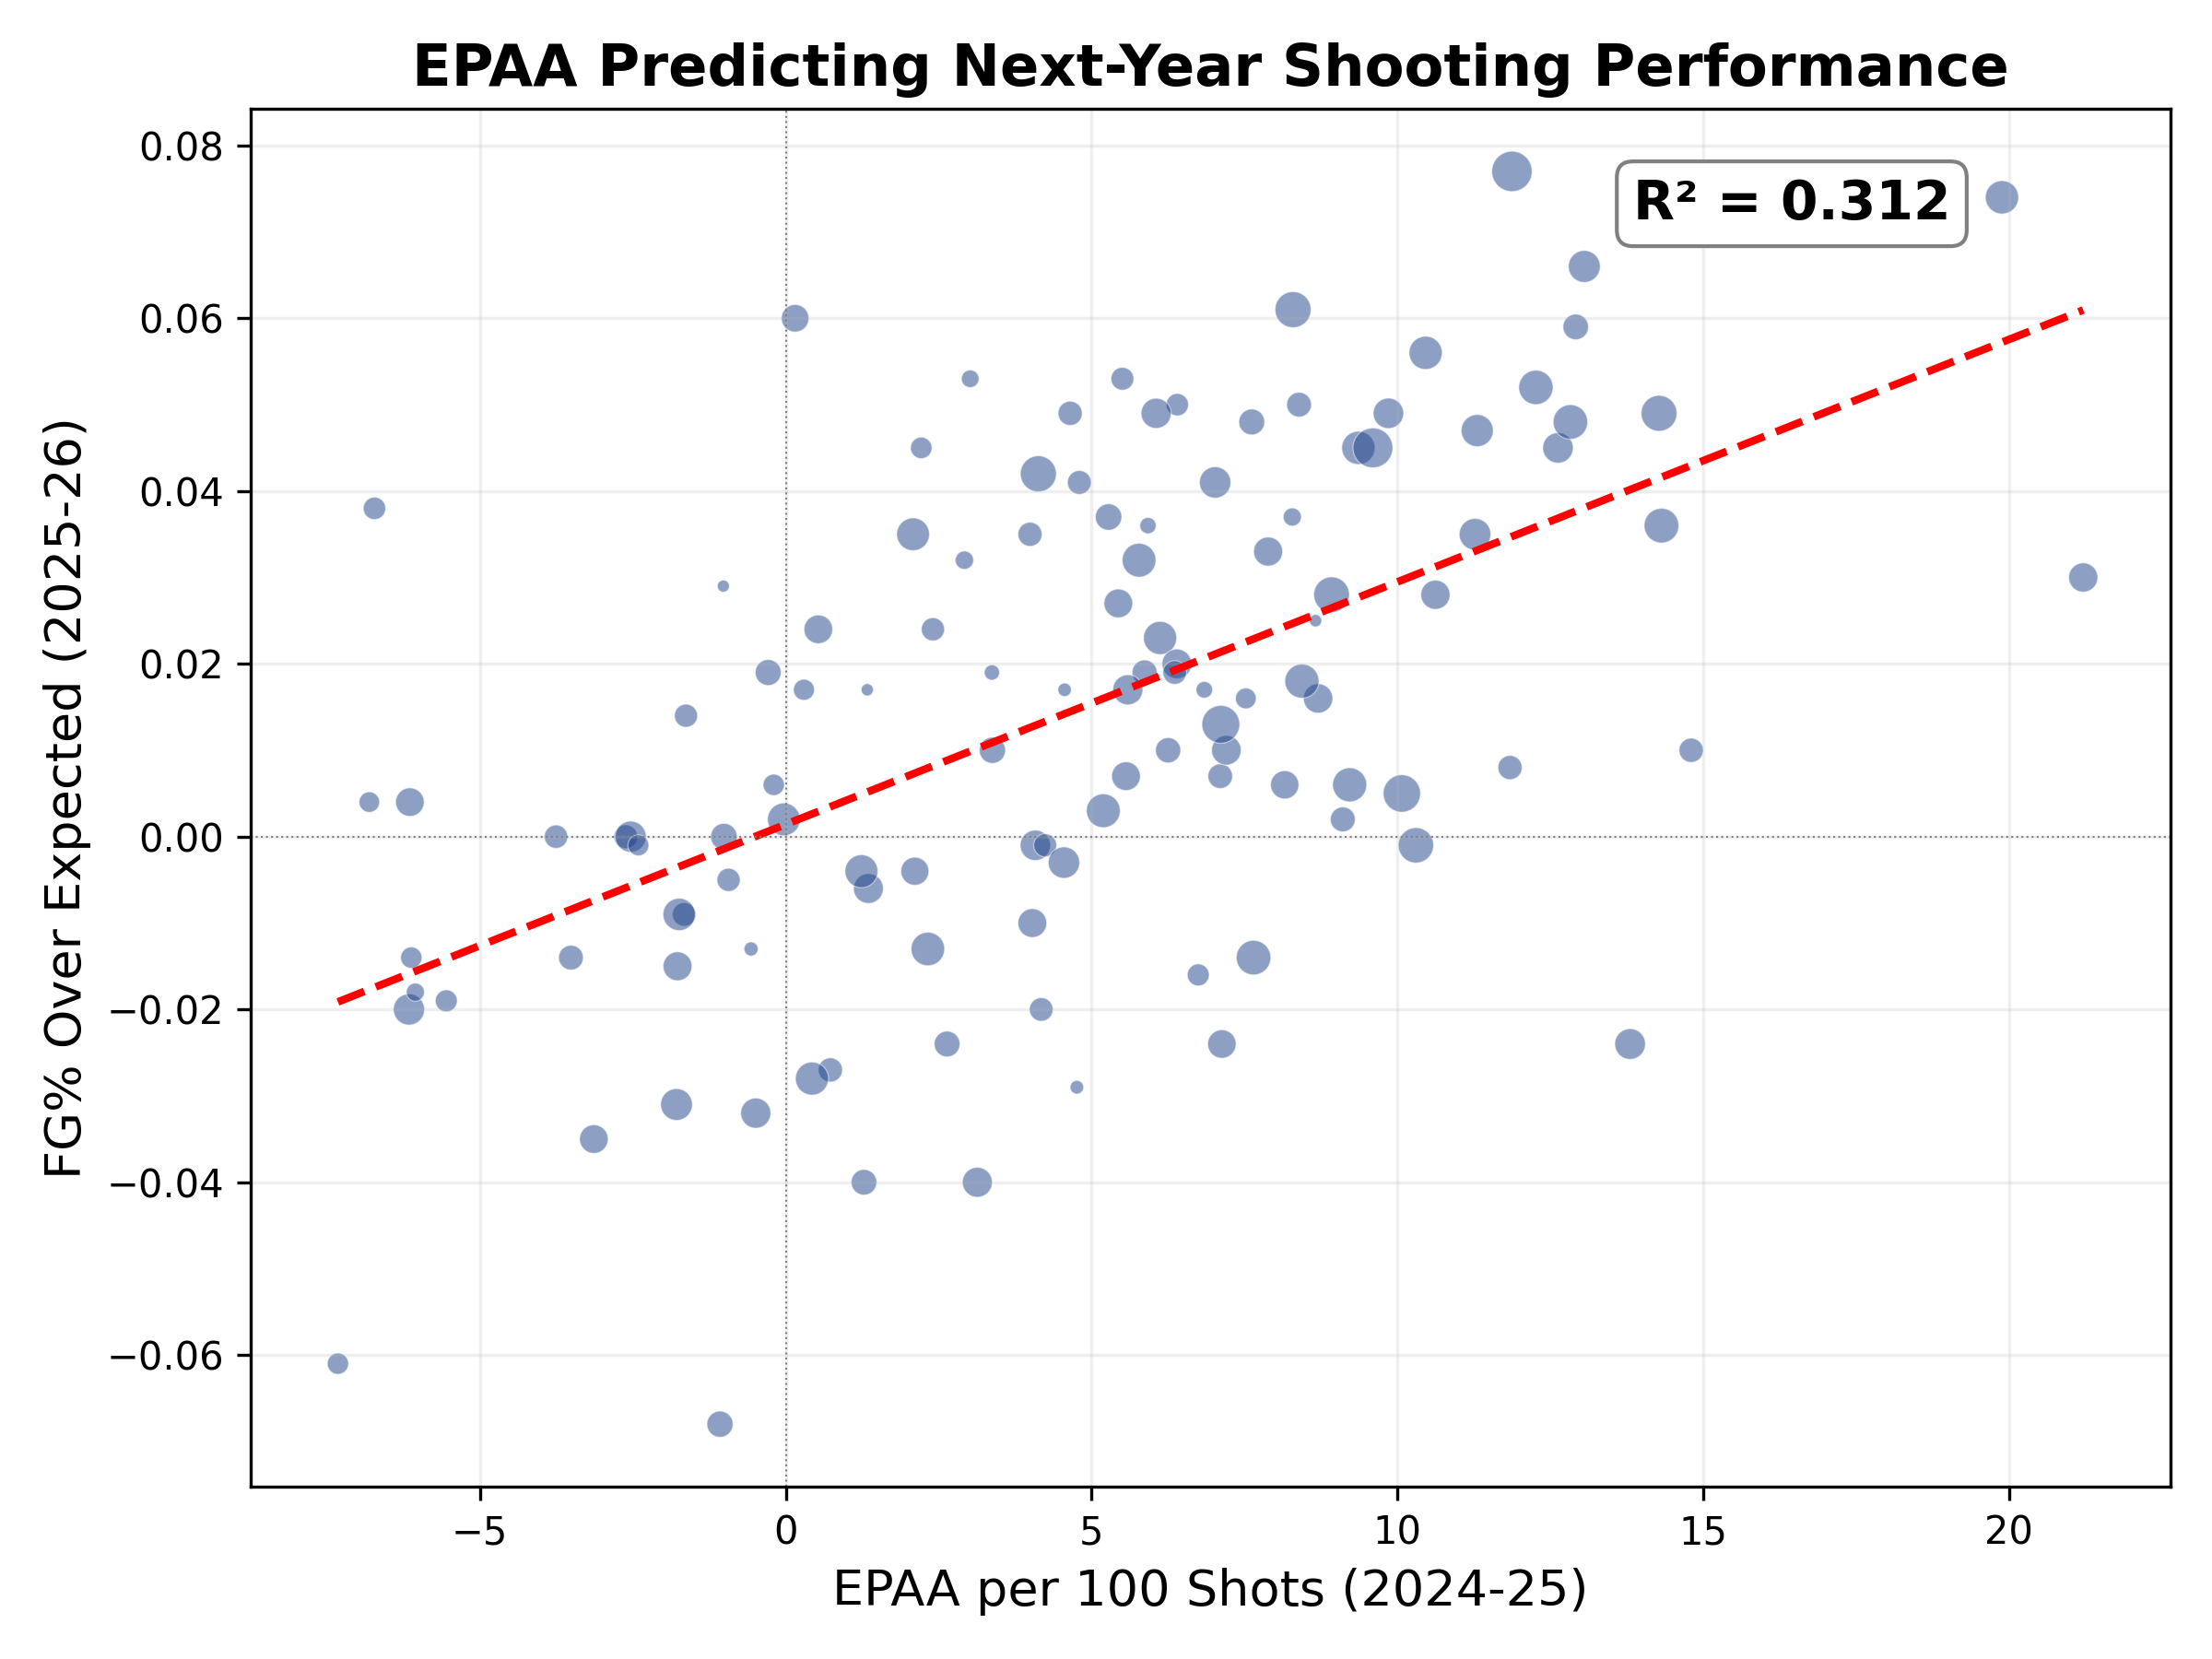
\includegraphics[width=\linewidth]{epaa_yoy_scatter.png}
\caption{\textbf{Year-over-Year Predictive Power} of EPAA for FG\% over expected.}
\end{minipage}
\end{figure}

\vspace{1ex}

\textbf{Key Findings}\\[0.5ex]
\begin{itemize}
\item EPAA rewards efficiency while penalizing inflated stats from easier shots.
\item Defender rankings reveal individual rim protection skill has tighter credible intervals than mid-range and 3-point defense (possibly more luck-driven).
\item Credible intervals for all defensive team parameters crossed 0.
\end{itemize}

\end{block}

%----------------------------------------------------------------------------------------
% CONCLUSION / FUTURE WORK / CODE
%----------------------------------------------------------------------------------------

\begin{block}{Conclusion}

EPAA demonstrates that a two-stage framework can \textbf{separate shot difficulty from shooting skill} with principled uncertainty quantification. The R² = 0.31 year-over-year correlation shows EPAA captures stable shooting talent signal.

\vspace{2ex}

\textbf{Limitations \& Future Direction}\\[0.5ex]
\begin{itemize}
\item The shot quality models are limited by the public NBA API. Detailed player tracking data could provide richer features and more accurate xFG estimations.
\item Future work will train models over multiple seasons of data. %This could allow for additional analysis such as aging effects on EPAA, year-over-year stability and predictive power of EPAA, the effect of changing teams on EPAA, as well as role-adjusted EPAA.
%\item The defensive parameters may be undervaluing defensive impact from a few perspectives. Because defender distance is included in the shot quality model, this may discount a defender's ability (or inability) to put himself in a position to contest a shot in the first place. 
\item Incorporating foul-drawing value would better capture a player's scoring impact.
\end{itemize}

\end{block}


%----------------------------------------------------------------------------------------
% REFERENCES
%----------------------------------------------------------------------------------------

% \begin{block}{References}
% 
% {\small
% \begin{enumerate}
% \item Gelman, A., et al. (2013). \textit{Bayesian Data Analysis}, 3rd ed. CRC Press.
% \item Osborn, C. (2024). Probabilistic modeling of true hitting talent in MLB. \textit{CSAS}.
% \item Franks, A., et al. (2015). Characterizing the spatial structure of defensive skill in professional basketball. \textit{Annals of Applied Statistics}, 9(1), 94--121.
% \item Cervone, D., et al. (2016). A multiresolution stochastic process model for predicting basketball possession outcomes. \textit{JASA}, 111(514), 585--599.
% \end{enumerate}
% }
% 
% \end{block}

%----------------------------------------------------------------------------------------

\end{column}
\begin{column}{\edgewid}\end{column}
\vspace{0.5in}
\end{columns}

\end{frame}

\end{document}
